\newpage
\section{Convolutional Neural Networks}
\begin{figure}[!htb]
    \centering
    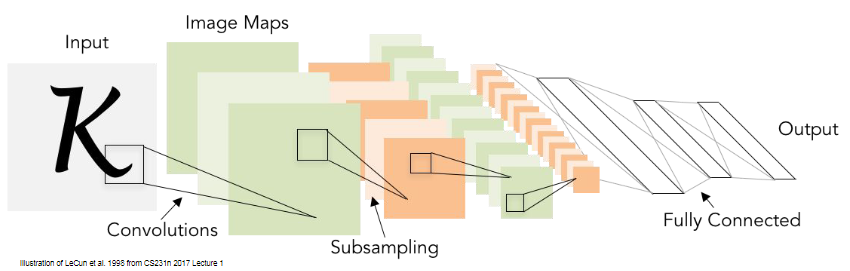
\includegraphics[width=0.42\textwidth]{pic/Lec5/CNN.png}
    \caption{CNN}
\end{figure}

\subsection{Fully Connected Layer}
Contains neurons that connect to the entire input volume, as in ordinary Neural Networks. $32\times 32\times 3$ image $\rightarrow$ stretch to $3072\times 1$

\begin{figure}[!htb]
    \centering
    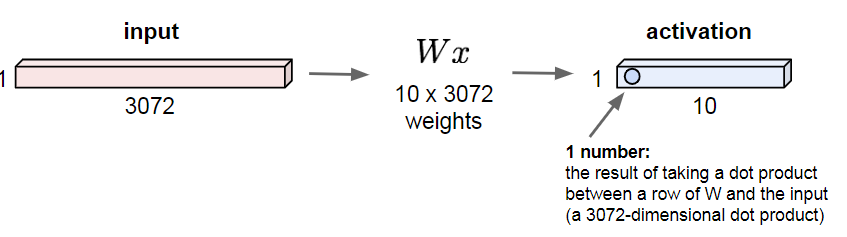
\includegraphics[width=0.42\textwidth]{pic/Lec5/FC.png}
    \caption{Fully Connected Layer}
\end{figure}

\subsection{Convolution Layer}
$32\times 32\times 3$ image $\rightarrow$ preserve spatial structure. 

Convolve the filter with the image i.e. ``slide over the image spatially, computing dot products''. Filters always extend the full depth of the input volume. The result is called activation map.

\begin{figure}[!htb]
    \centering
    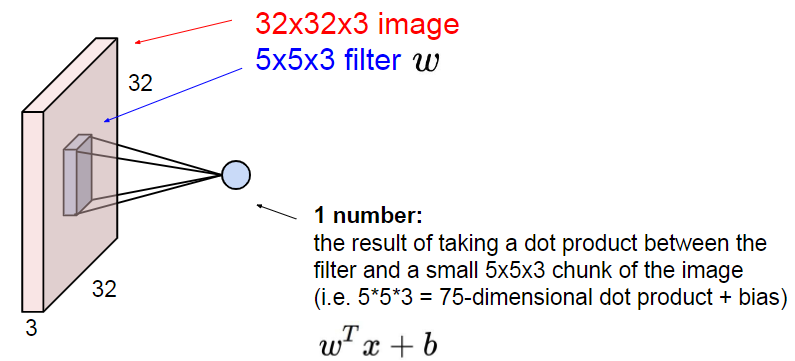
\includegraphics[width=0.42\textwidth]{pic/Lec5/C.png}
    \caption{Convolution Layer}
\end{figure}

ConvNet is a sequence of Convolution Layers, interspersed with activation functions. 

\begin{figure}[!htb]
    \centering
    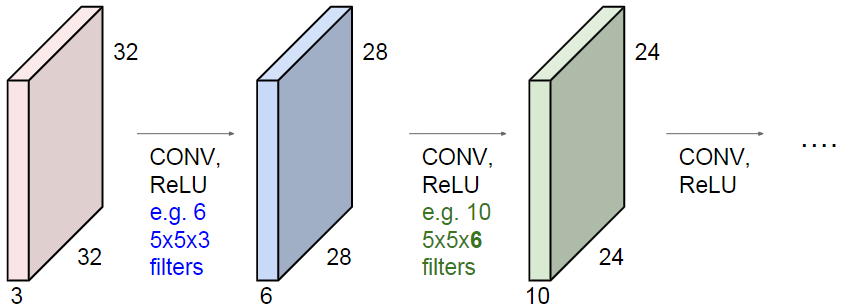
\includegraphics[width=0.42\textwidth]{pic/Lec5/ConvNet.png}
    \caption{ConvNet}
\end{figure}

We call the layer convolutional because it is related to convolution of two signals:
\begin{align*}
    f(x,y)*g(x,y)=\sum_{n_1=-\infty}^{\infty}\sum_{n_2=-\infty}^{\infty}f(n_1, n_2)\cdot g(x-n_1, y-n_2)
\end{align*}

\textbf{Summary}
\begin{itemize}
    \item 输入体积 $W_1\times H_1 \times  D_1$
    \item 超参数
    \begin{itemize}
        \item filters 数量 $K$
        \item receptive field (感受野) $F$
        \item stride (步长) $S$
        \item zero padding 数量 $P$
    \end{itemize}
    \item 输出体积 $W_2\times H_2 \times  D_2$, where
    \begin{align*}
        W_2&=\frac{W_1 -F +2P}{S}+1\\
        H_2&=\frac{H_1 -F +2P}{S}+1\\
        D_2&=K
    \end{align*}
    \item 因为参数共享, 每个 filter 有 $F\cdot F\cdot D_1$ weights, 所以一共 $(F\cdot F\cdot D_1)\cdot K$ weights 与 $K$ biases. 
\end{itemize}

$1\times 1$ convolution layers 可以改变深度. 

\subsection{Pooling layer}
Makes the representations smaller and more manageable. Operates over each activation map independently. 

\begin{figure}[!htb]
    \centering
    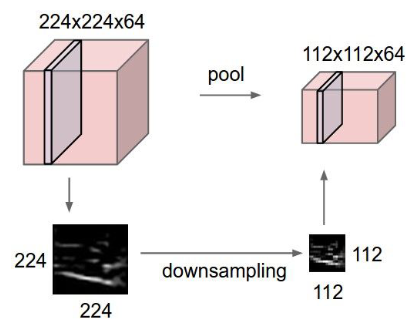
\includegraphics[width=0.309\textwidth]{pic/Lec5/Pooling layer.png}
    \caption{Pooling layer}
\end{figure}

\textbf{Summary}
\begin{itemize}
    \item 输入体积 $W_1\times H_1 \times  D_1$
    \item 超参数
    \begin{itemize}
        \item receptive field (感受野) $F$
        \item stride (步长) $S$
    \end{itemize}
    \item 输出体积 $W_2\times H_2 \times  D_2$, where
    \begin{align*}
        W_2&=\frac{W_1 -F}{S}+1\\
        H_2&=\frac{H_1 -F}{S}+1\\
        D_2&=D_1
    \end{align*}
    \item 没有参数, 因为是个固定的函数. 
\end{itemize}

